\documentclass{article} % For LaTeX2e
\usepackage{nips15submit_e,times}
\usepackage{amsmath}
\usepackage{hyperref}
\usepackage{url}
\usepackage{graphicx}
%\documentstyle[nips14submit_09,times,art10]{article} % For LaTeX 2.09


\title{Approximately Bayesian Demixing with Neural Networks \\ David Halpern}


\author{
David Halpern\\
Department of Psychology\\
New York University\\
\texttt{david.halpern@nyu.edu} \\
}

\newcommand{\fix}{\marginpar{FIX}}
\newcommand{\new}{\marginpar{NEW}}

\nipsfinalcopy % camera-ready version

\begin{document}


\maketitle


\section{Introduction}

\section{Methods}
In order to test the performance of the neural networks, we generated stimuli according to the following statistical model. We used two stimuli for all but the last experiment when only one was used. $s_1$ was drawn discrete uniform distribution over the interval [-60, 60]. $s_2$ was then drawn from the interval [$s_1$, 60]. Finally, we generated a neural response with Poisson noise and tuning curves were given by linear combinations of the responses to each individual input. In notation:
\begin{equation}
	\mathbf{r} = \text{Poisson}(\sum_i g_i \mathbf{f}(s_i))
\end{equation}
where $\mathbf{r}$ is the vector of spike counts on a particular trial, $\mathbf{f}$ is the vector of tuning curves for individual stimuli, $g_i$ is the gain for the $i$th stimulus and $s_i$ is the orientation of the $i$th stimulus. Gain here can be thought of as being the neural representation of the contrast of the stimulus (although could be modulated by many other things such as attention).
Each tuning curve is given by
\begin{equation}
	f_i = e^\frac{(s - s_{\text{pref}_i})^2}{2 \sigma_{tc}^2}
\end{equation}
\begin{figure}[h]
\centering
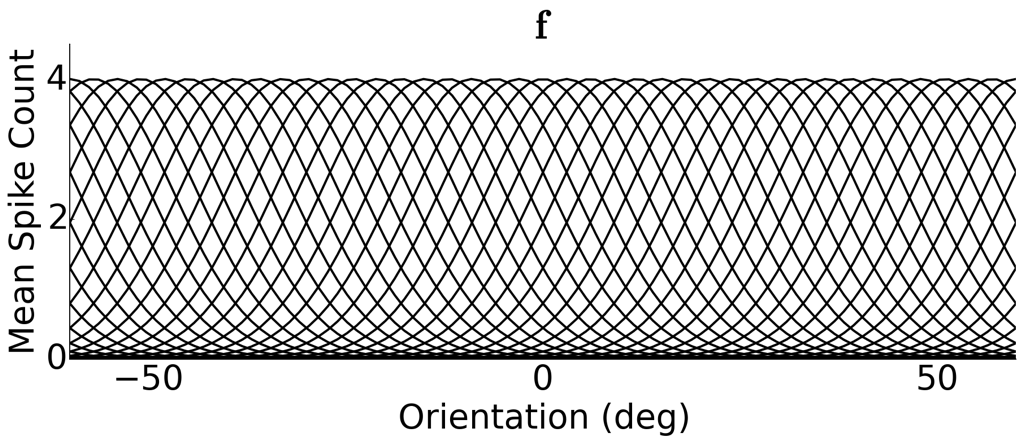
\includegraphics[width = \textwidth]{Tuning_Curves.png}
\caption{Mean firing rate of every neuron in the input population as a function of stimulus input}
\end{figure}
\\
All of the $s_{\text{pref}_i}$ were evenly tiled over [-90, 90]. This was larger than the range of possible stimuli in order to mitigate edge effects. In our simulations we used 61 neurons and $\sigma_{tc}$ was set to 10.
\\
\\
We computed the posterior mean on every trial in order to have a baseline for comparison with the networks. We computed this using a grid approximation where we computed the unnormalized posterior at all the possible combinations of $s_1$ and $s_2$.
\\
\\
Throughout, we investigate the performance of a three layer nonlinear network with an input layer, a hidden layer and an output layer (which produces the estimates). The input layer consisted of the 61 neurons described above. The neural network then included a hidden layer with 20 units which are fully connected to all of the input units. The activation function for the hidden units is given by a linear combination of the inputs followed by a pointwise nonlinearity. Again, in notation:
\begin{equation}
	\mathbf{r}_{\text{hid}} = \sigma(\mathbf{Wr + b})
\end{equation}
Where $\mathbf{r}_{\text{hid}}$ is the vector of activations, $W$ is the matrix of weights and $b$ is a vector of bias terms. For the nonlinearity, we used Rectified Linear Units \cite{NairH10} which are defined as:
\begin{equation}
	\sigma(x) = \max(0, x)
\end{equation}
Finally, the network outputs (estimates of $\mathbf{s}$) were linear combinations of the hidden unit activations,  
\begin{equation}
	\mathbf{\hat{s}} = \mathbf{W_{\text{hid}} r_{\text{hid}}}
\end{equation}
Where $\mathbf{W_{\text{hid}}}$ is the weight matrix. For all except the last problem there were two outputs, in the last problem there was only one. 
In order to train these networks, we used stochastic gradient descent with minibatches of size 20. We used a learning rate of .0001, a momentum of .9 \cite{Sutskever2013} and RMSProp \cite{Tieleman2012} with a rho parameter of .9 and trained the networks for 100 epochs. For every problem, we gave the network 270,000 training trials that were generated from the statistical model stated above. We implemented the neural network using Theano.
\\
\\
\section{Experiments}
To give the network the best chance at a high performance, we first conducted an experiment where it would not have to marginalize over gain. Therefore, we only generated training trials for a network with a single pair of gains. During the test phase, we gave only trials with that exact set of gains. For a fair comparison to the posterior, we computed the posterior mean using that set of gains rather than marginalizing over gain. For plotting and comparison purposes, we fixed the first stimulus ($s_1$) at a single orientation and then compared the network and posteriors estimates of $s_2$ over a range of differences in orientation (here from 0 to 30). We generated 4500 trials at ($s_1, s_2$) pair and tested the networks and the posterior on the same set of trials. In order to better understand the performance of the network relative to that of the posterior mean, we split up the errors made by both into a bias term and a variance (here standard deviation) term. Since the stochastic training algorithm can result in a different set of weights depending on the order of training examples and we wanted to get a sense of average network performance, we generated 200 networks per gain combination and computed the bias and variance for each one. For visualization purposes, we show plus/minus one standard deviation of the neural network's bias and standard deviation terms, shown in purple in the figure. Since the posterior remains the same, it is simply a black line in each plot. It is clear that the network is not only well approximating the posterior but also qualitatively has bias and variance as a function of the difference in the stimuli orientation.
\begin{figure}[h]
\centering
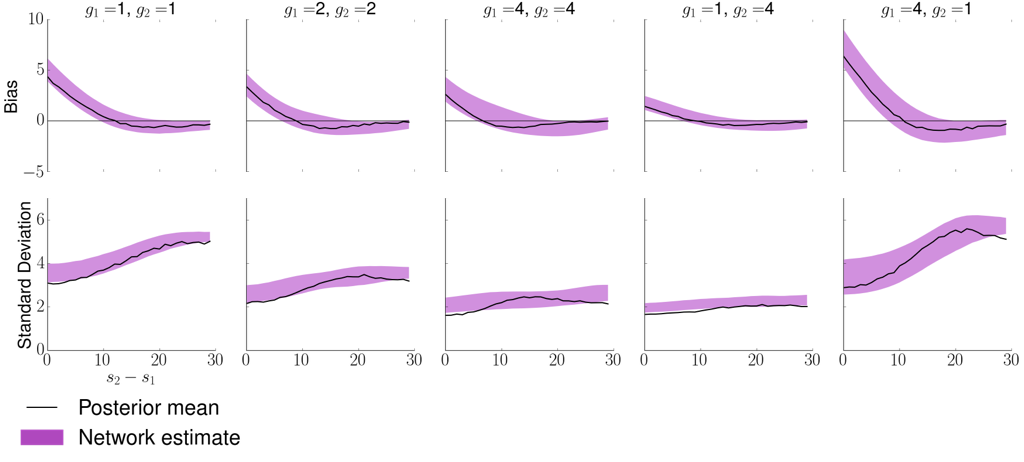
\includegraphics[width = \textwidth]{Fixed_Gains.png}
\caption{Error of the posterior mean and network estimates in the fixed gains condition. The pair of gains used for training the networks, computing the posterior and testing for each plot is listed above the plot.}
\end{figure}
\\
In the real world, brains are confronted with a variable set of contrasts and so must attempt to ignore contrast in order to decode orientation from an input population like ours. Therefore, we now add a prior over gain which is uniform over all pairs of {1, 2, 4}. In the posterior computation, we now marginalize over this prior. For the network, we simply train the network using all combinations rather than just a single set of gains. We keep the training set at 270,000 trials and use 30,000 trials for each gain combination. We again split up the test performance by gain combination but since the networks were trained on all the gain combinations we use the same networks for all five plots. The standard deviations on the network error are computed over the performance of 400 networks. Again, the networks well approximate the posterior and seem to learn similar errors
\begin{figure}[h]
\centering
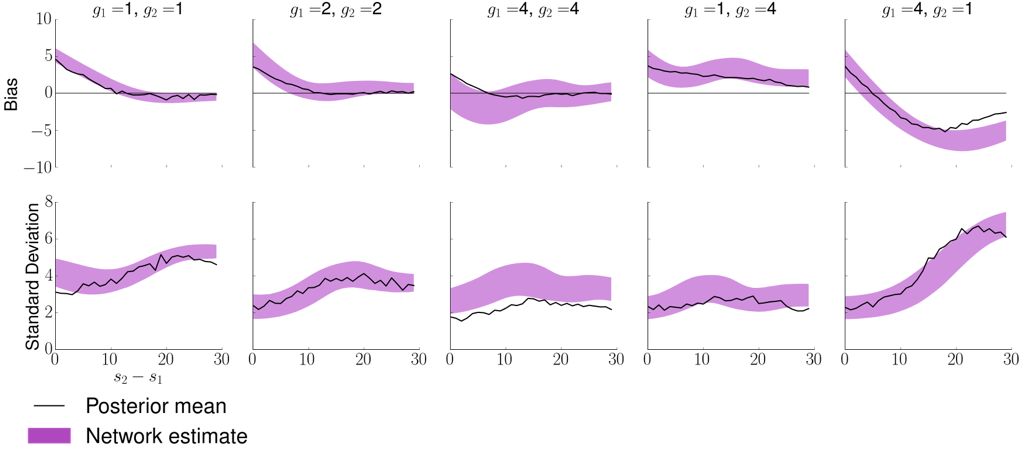
\includegraphics[width = \textwidth]{Variable_Gains.png}
\caption{Error of the posterior mean and network estimates in the variable gains condition. The pair of gains used for testing in each plot is listed above the plot. However, the same networks are used for all plots and in all plots the posterior mean marginalizes over gain.}
\end{figure}
\\
We wanted to check whether it was absolutely necessary to provide the network with all of the gain combinations. Since the network was trying to approximate a function, it is possible that it could interpolate, given some training data at the highest and lowest gain combinations. This generalization to unseen stimuli is a requirement for a brain in an uncertain world and the network's good performance on this task is surprising and suggests that it is truly approximating the posterior. The standard deviations on the network error are again computed over the performance of 400 networks. Like above, the same networks are used for all five plots. The posterior mean is exactly the same as in the variable gains condition since the problem statement hasn't changed.
\begin{figure}[h]
\centering
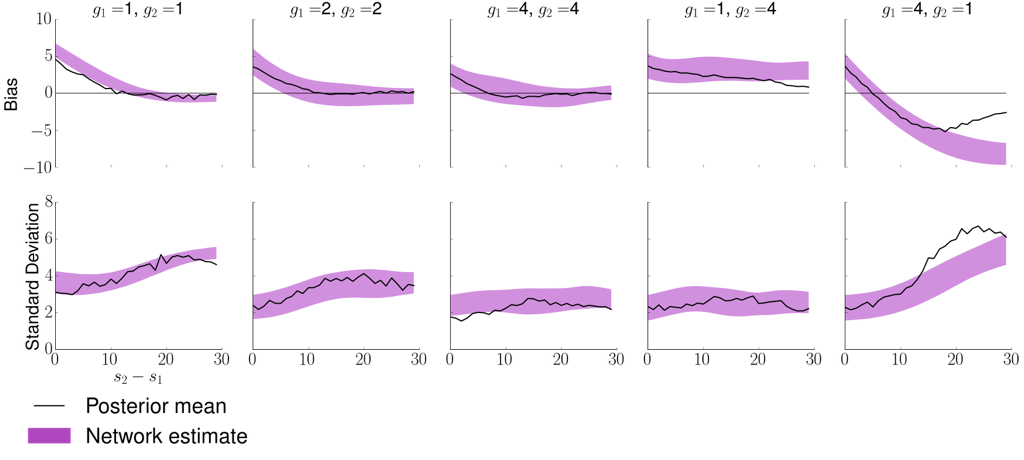
\includegraphics[width = \textwidth]{High-Low_Gains.png}
\caption{Error of the posterior mean and network estimates in the generalization condition. The pair of gains used for testing in each plot is listed above the plot. However, the same networks are used for all plots.}
\end{figure}

\bibliography{abdnn}
\bibliographystyle{plain}

\end{document}